\chapter{สถาปัตยกรรม AIoT วิทัศน์คอมพิวเตอร์ และเกษตรแม่นยำสำหรับไมโครไบโอม}
\label{ch:aiot_precision}

\begin{keyconcept}[แนวคิดสำคัญของบทที่ 10]
การปฏิวัติการเกษตรสู่ยุคดิจิทัล (Agriculture 4.0/5.0) ก้าวข้ามจากการตรวจวัดค่าเคมีกายภาพแบบแยกส่วน สู่การเชื่อมโยงระบบโทรมาตรภาคสนาม (Field Telemetry)\index{โทรมาตรแปลงเกษตร (Field Telemetry)} เข้ากับพลวัตของไมโครไบโอมดินและสรีรวิทยาพืชผ่านสถาปัตยกรรม \textbf{AIoT (Artificial Intelligence of Things)\index{AIoT (Artificial Intelligence of Things)}} การบูรณาการเซนเซอร์ดินอเนกประสงค์ (RS485 Modbus RTU 7-in-1)\index{โพรโทคอล Modbus RTU}\index{RS485 Differential Signaling} ร่วมกับไมโครคอนโทรลเลอร์ ESP32\index{ESP32-S3 Microcontroller} และเครือข่ายสัญญาณระยะไกล LoRaWAN\index{LoRaWAN (Long Range Wide Area Network)} ทำให้สามารถติดตามความชื้น อุณหภูมิ ดัชนีการนำไฟฟ้า (EC) และสารอาหารดินแบบเรียลไทม์ ขณะเดียวกัน การประยุกต์ใช้โมเดลวิทัศน์คอมพิวเตอร์ขนาดย่อมเยา (Edge AI: YOLOv8-Nano, MobileNetV4)\index{การตรวจจำแนกโรคพืชด้วย Edge AI}\index{YOLOv8-Nano Deep Learning}\index{MobileNetV4} และอัลกอริทึมการเรียนรู้ของเครื่อง (Machine Learning: Random Forest)\index{Random Forest Regression} ช่วยให้สามารถประเมินดัชนีความรุนแรงของโรคพืชและควบคุมการปล่อยชีวภัณฑ์ PGPR แบบแปรผันตามพื้นที่จริงได้อย่างแม่นยำ
\end{keyconcept}

\begin{figure}[ht]
    \centering
    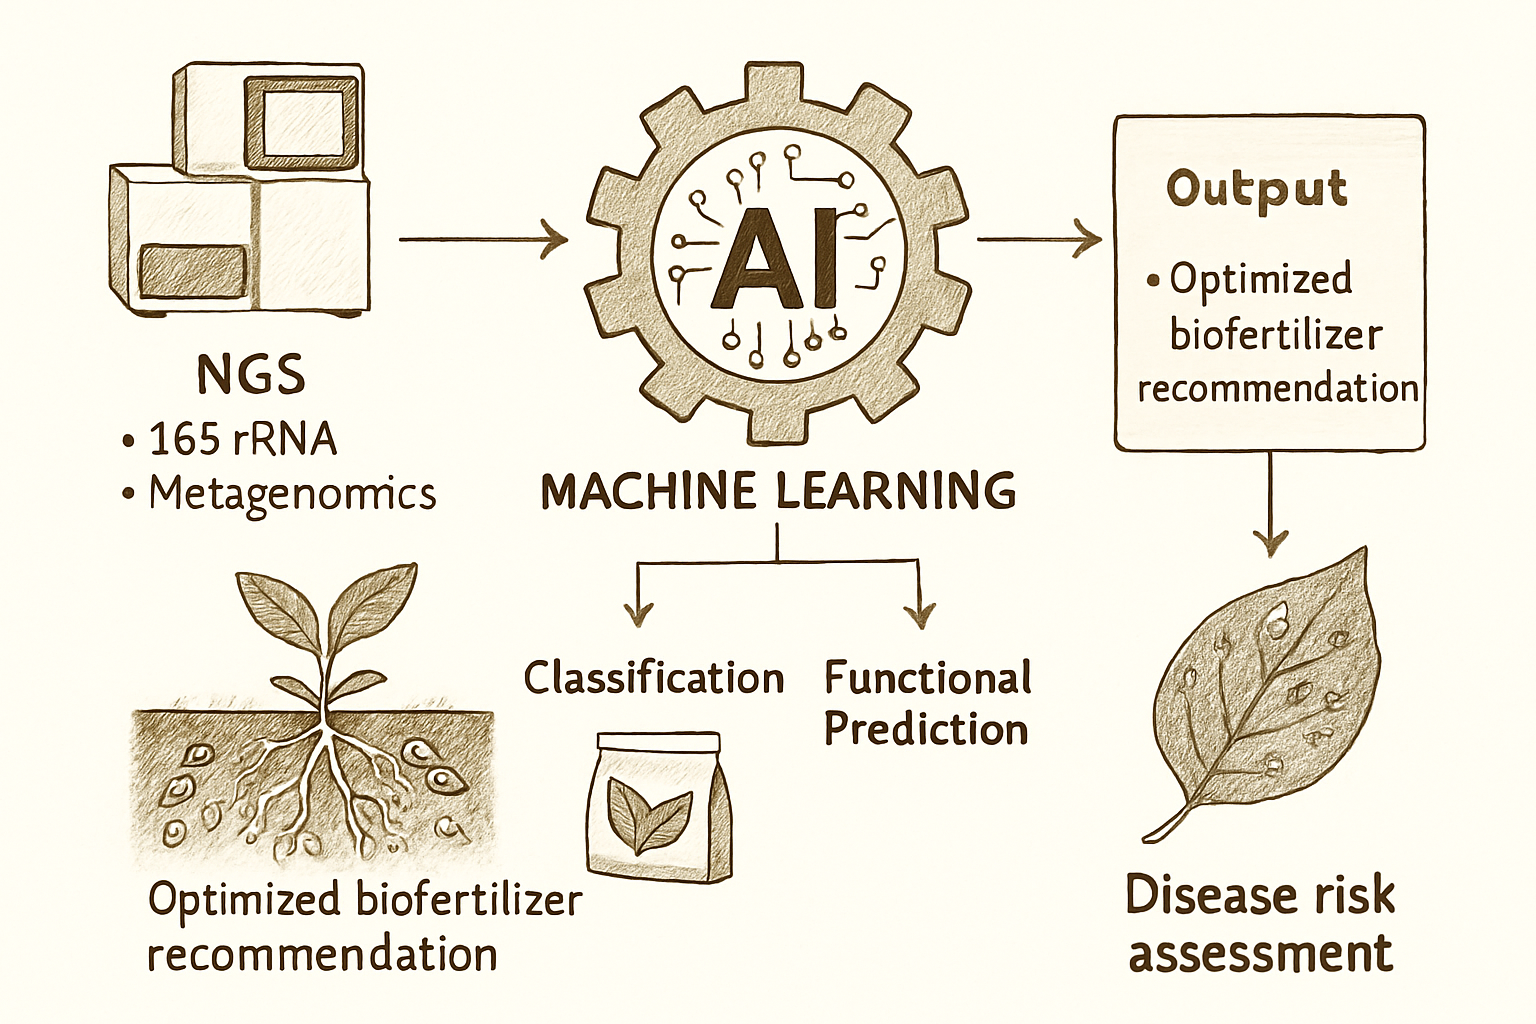
\includegraphics[width=0.85\textwidth]{assets/ch10_ai_telemetry.png}
    \caption{สถาปัตยกรรมระบบนิเวศ AIoT ในแปลงเกษตรอัจฉริยะ แสดงเซนเซอร์ดิน RS485 Modbus RTU โหนดประมวลผลไมโครคอนโทรลเลอร์ ESP32 การส่งผ่านข้อมูลด้วยสัญญาณ LoRaWAN เข้าสู่แดชบอร์ดคลาวด์ และโมเดล Edge AI ตรวจจำแนกโรคพืชและควบคุมการฉีดพ่นชีวภัณฑ์อัตโนมัติ}
    \label{fig:ch10_aiot_architecture}
\end{figure}

\section*{วัตถุประสงค์การเรียนรู้ประจำบท}
เมื่อศึกษาบทเรียนนี้จบแล้ว นักศึกษาสามารถ:
\begin{enumerate}
    \item อธิบายสถาปัตยกรรมระบบโทรมาตร AIoT และโปรโตคอลการสื่อสารอุตสาหกรรม RS485 Modbus RTU สำหรับเซนเซอร์ดิน
    \item ถอดรหัสโครงสร้างเฟรมข้อมูลฐานสิบหก (Hexadecimal Frame) และการคำนวณรหัสตรวจสอบความถูกต้อง CRC16 ของเซนเซอร์ดิน
    \item วิเคราะห์การประยุกต์ใช้อัลกอริทึมการเรียนรู้ของเครื่อง (Random Forest / LightGBM) เพื่อสร้างแบบจำลองทำนายพลวัตของจุลินทรีย์ในดิน
    \item อธิบายสถาปัตยกรรมโครงข่ายประสาทเทียมแบบขนาดย่อมเยา (Lightweight Edge AI: YOLOv8-Nano, MobileNetV4) สำหรับการตรวจจับโรคพืช
    \item คำนวณเมทริกซ์ความสับสน (Confusion Matrix) ค่าความแม่นยำ (Precision) ความระลึก (Recall) และ F1-Score ของโมเดลจำแนกโรคพืช
\end{enumerate}

\section{สถาปัตยกรรมฮาร์ดแวร์และโทรมาตร AIoT ในแปลงเกษตร}

ระบบฟาร์มอัจฉริยะที่เชื่อมโยงกับชีววิทยาของจุลินทรีย์ดิน ประกอบด้วยโครงสร้างพื้นฐานทางวิศวกรรม 4 ระดับชั้น (4-Tier Architecture):

\begin{figure}[ht]
\centering
\begin{tikzpicture}[node distance=1.6cm, auto,
    layer/.style={rectangle, draw, fill=teal!15, text width=10.5cm, rounded corners, minimum height=1.0cm, align=left},
    arrow/.style={thick, <->, >=stealth}]
    
    \node [layer] (l1) {\textbf{1. Perception Layer (ชั้นตรวจวัด):} หัววัดดิน 7-in-1 (RS485 Modbus RTU), กล้องตรวจการณ์ Multispectral, เซนเซอร์สภาพอากาศ microclimate};
    \node [layer, below of=l1] (l2) {\textbf{2. Edge Computing Layer (ชั้นประมวลผลปลายทาง):} ไมโครคอนโทรลเลอร์ ESP32-S3, ชิปประมวลผล NPU (Coral Edge TPU / Raspberry Pi 5)};
    \node [layer, below of=l2] (l3) {\textbf{3. Network Layer (ชั้นสื่อสาร):} โครงข่าย LoRaWAN (ความถี่ $920-925\text{ MHz}$), NB-IoT, 4G LTE Gateway};
    \node [layer, below of=l3] (l4) {\textbf{4. Application \& Cloud Layer (ชั้นแอปพลิเคชัน):} MQTT Broker, แดชบอร์ด Grafana, ระบบฐานข้อมูล TimescaleDB, โมเดลพยากรณ์ AI};
    
    \draw [arrow] (l1) -- (l2);
    \draw [arrow] (l2) -- (l3);
    \draw [arrow] (l3) -- (l4);
\end{tikzpicture}
\caption{สถาปัตยกรรม 4 ระดับชั้นของระบบ AIoT สำหรับการเกษตรแม่นยำและการติดตามไมโครไบโอม}
\label{fig:aiot_4tier}
\end{figure}

\subsection{1. โปรโตคอลการสื่อสารอุตสาหกรรม RS485 Modbus RTU}
ในสภาพแปลงเกษตรกรรมที่มีสายสัญญาณยาวหลายสิบเมตรและมีสัญญาณรบกวนแม่เหล็กไฟฟ้า การใช้สัญญาณแอนะล็อกทั่วไปจะเกิดความคลาดเคลื่อนสูง มาตรฐานอุตสาหกรรมจึงเลือกใช้ **RS485 Differential Signaling** ทำงานร่วมกับโปรโตคอล **Modbus RTU**:
\begin{itemize}
    \item ส่งสัญญาณแบบ Differential ผ่านคู่สายเกลียวบิด (A และ B) ต้านทานสัญญาณรบกวนได้สูง
    \item ส่งข้อมูลเป็นไบนารีฐานสิบหก (Hexadecimal) ประกอบด้วย:
    $$\underbrace{\text{[Slave ID]}}_{1\text{ Byte}} + \underbrace{\text{[Function]}}_{1\text{ Byte}} + \underbrace{\text{[Start Reg]}}_{2\text{ Bytes}} + \underbrace{\text{[Length]}}_{2\text{ Bytes}} + \underbrace{\text{[CRC16]}}_{2\text{ Bytes}}$$
    \item ฟังก์ชันโค้ดมาตรฐานสำหรับการอ่านค่ารีจิสเตอร์เซนเซอร์คือ **0x03 (Read Holding Registers)**
\end{itemize}

\subsection{2. ไมโครคอนโทรลเลอร์และการส่งสัญญาณระยะไกล LoRaWAN}
ไมโครคอนโทรลเลอร์ **ESP32** ทำหน้าที่เป็นโหนดประมวลผลระดับแปลง (Edge Node) เชื่อมต่อกับบอร์ดแปลงสัญญาณ RS485-to-TTL ควบคุมการเปิด-ปิดแหล่งจ่ายไฟเซนเซอร์เพื่อประหยัดพลังงานจากแผงโซลาร์เซลล์ จากนั้นส่งแพ็กเก็ตข้อมูลผ่านโมดูล **LoRa (Long Range)** ซึ่งสามารถส่งสัญญาณได้ไกลกว่า $5 - 10\text{ กิโลเมตร}$ ในพื้นที่สวนผลไม้โดยไม่ต้องพึ่งพาซิมการ์ดในทุกต้น

\section{การเรียนรู้ของเครื่อง (Machine Learning) กับพลวัตไมโครไบโอมดิน}

ข้อมูลกายภาพและเคมีจากเซนเซอร์ดิน (อุณหภูมิ, ความชื้น, EC, pH, N, P, K) มีสหสัมพันธ์โดยตรงต่ออัตราการรอดชีวิตและกิจกรรมเมแทบอลิซึมของจุลินทรีย์ดิน \cite{thassana_2026, pmid41735330}:

\subsection{1. อัลกอริทึม Random Forest Regression}
Random Forest เป็นโมเดลกลุ่มรวม (Ensemble Learning) ที่สร้างจากต้นไม้ตัดสินใจ (Decision Trees) จำนวนมาก โดยใช้เทคนิค Bootstrap Aggregating (Bagging) เหมาะอย่างยิ่งสำหรับข้อมูลการเกษตรที่มีลักษณะไม่เป็นเชิงเส้น (Non-linear) และมีสัญญาณรบกวน:
\begin{itemize}
    \item ทำนายปริมาณประชากรจุลินทรีย์ส่งเสริมการเติบโตพืช (PGPR Viable Count)
    \item คำนวณดัชนีการทำงานของเอนไซม์ในดิน (Dehydrogenase / Urease Activity)
    \item ระบุค่าความสำคัญของตัวแปร (Feature Importance) เพื่อระบุว่าปัจจัยทางกายภาพใดจำกัดการเติบโตของจุลินทรีย์มากที่สุด
\end{itemize}

\subsection{2. การทำนายความเสี่ยงการระบาดของโรคพืชล่วงหน้า}
การผสานข้อมูลความชื้นในดินที่สูงต่อเนื่อง ($> 85\%$) อุณหภูมิช่วง $26 - 30^\circ\text{C}$ ร่วมกับระยะเวลาใบเปียกชื้น (Leaf Wetness Duration) ผ่านแบบจำลองการจำแนกประเภท (Binary Classification: Support Vector Machine หรือ Gradient Boosting) ช่วยเตือนภัยล่วงหน้า $3 - 5\text{ วัน}$ ก่อนที่เชื้อรา \organism{Phytophthora} จะสร้างซูโอสปอร์เข้าทำลายรากทุเรียน

\begin{application}[การติดตั้งและทดสอบระบบโทรมาตร AIoT ในแปลงวิจัย มรภ.รำไพพรรณี จ.จันทบุรี]
จากงานวิจัยของ Thassana และคณะ (2026) \cite{thassana_2026}, Tsana \& Chantamalee (2026) \cite{tsana2026edge}, และ Thassana \& Jantamalee (2024, 2025) \cite{thassana_2024_soil, thassana_2025_aiot} ได้ดำเนินโครงการนำร่องติดตั้งระบบโครงข่ายเซนเซอร์ดินและสถานีโทรมาตรไร้สาย LoRaWAN ในแปลงวิจัยทุเรียนขนาด 50 ไร่ ณ มหาวิทยาลัยราชภัฏรำไพพรรณี จ.จันทบุรี:\index{งานวิจัย RBRU!โทรมาตรแปลงวิจัยทุเรียน}
\begin{itemize}
    \item \textbf{การเก็บข้อมูลกายภาพเคมีดิน:} ติดตั้งโหนดเซนเซอร์ 7-in-1 (Soil Moisture, Temp, EC, pH, N, P, K) จำนวน 20 จุด เชื่อมต่อผ่านคู่สาย RS485 Modbus RTU เข้ากับไมโครคอนโทรลเลอร์ ESP32-S3 ส่งสัญญาณด้วยโมดูล LoRa SX1262 (ย่านความถี่ 920--925 MHz) ครอบคลุมรัศมี 4.2 กิโลเมตร ภายใต้สภาพสวนผลไม้ที่มีร่มเงาหนาทึบ
    \item \textbf{สมรรถนะการทำนายด้วย Random Forest:} แบบจำลองสามารถทำนายปริมาณประชากรแบคทีเรียตรึงไนโตรเจนและ PGPR ในเขตรากพืชได้แม่นยำสูง ($R^2 = 0.942$, $\text{RMSE} = 0.28\text{ log CFU/g}$) โดยพบว่าความชื้นในดินและค่า pH เป็นตัวแปรที่มีค่า Feature Importance\index{Feature Importance} สูงสุด ($42\%$ และ $28\%$ ตามลำดับ)
    \item \textbf{การตอบสนองแบบเรียลไทม์:} เมื่อระบบตรวจพบสภาวะเสี่ยง (ความชื้นดิน $>80\%$ ร่วมกับอุณหภูมิ $27-30^\circ\text{C}$ นานเกิน 48 ชม.) อัลกอริทึมจะสั่งการเปิดวาล์วระบบน้ำหยดเพื่อปล่อยสารชีวภัณฑ์ \organism{Trichoderma} และ \organism{Bacillus} ไปยังโคนต้นที่มีความเสี่ยงสูงโดยอัตโนมัติ ช่วยลดความสูญเสียจากโรคเน่าได้ร้อยละ 58
\end{itemize}
\end{application}

\section{Edge AI วิทัศน์คอมพิวเตอร์และการตรวจจำแนกโรคพืช}
\index{Edge AI}\index{Computer Vision}\index{OpenCV}

การตรวจวินิจฉัยโรคพืชในอดีตต้องส่งตัวอย่างเข้าห้องปฏิบัติการหรือส่งภาพขึ้นคลาวด์ ซึ่งไม่ตอบโจทย์ในพื้นที่ห่างไกลที่ไม่มีสัญญาณอินเทอร์เน็ต เทคโนโลยี **Edge AI** นำโครงข่ายประสาทเทียมเชิงลึก (Deep Learning) ที่ผ่านการบีบอัดขนาดลงมาติดตั้งบนอุปกรณ์ภาคสนาม \cite{chouhan2020deep, reddy2024edgeai, tsana2026edge}:

\subsection{1. สถาปัตยกรรม YOLOv8-Nano และ MobileNetV4}
\index{Deep Learning!MobileNetV4}\index{Deep Learning!YOLOv8}\index{Depthwise Separable Convolution}\index{Model Quantization}
\begin{itemize}
    \item \textbf{MobileNetV4:} ใช้ Depthwise Separable Convolutions ร่วมกับ inverted residual blocks ทำให้ลดจำนวนพารามิเตอร์ลงเหลือต่ำกว่า 3 ล้านพารามิเตอร์ ใช้หน่วยความจำแฟลชเพียง $10 - 15\text{ MB}$
    \item \textbf{YOLOv8-Nano (YOLOv8n):} สถาปัตยกรรม Object Detection แบบ Single-Stage ตรวจจับรอยแผลโรคพืช (Bounding Boxes) พร้อมจำแนกชนิดเชื้อก่อโรคได้พร้อมกัน ด้วยความเร็วมากกว่า 30 เฟรมต่อวินาที (FPS) บนบอร์ดคอมพิวเตอร์ขนาดจิ๋ว
    \item \textbf{Model Quantization (Post-Training Quantization: INT8):} การแปลงค่าน้ำหนักเวต (Weights) จากทศนิยม 32-บิต (FP32) เป็นจำนวนเต็ม 8-บิต (INT8) ช่วยลดขนาดโมเดลลง $75\%$ และเร่งความเร็วในการประมวลผลขึ้น $3 - 4$ เท่า โดยไม่สูญเสียความแม่นยำอย่างมีนัยสำคัญ
\end{itemize}

\subsection{2. การประมวลผลภาพและการตัดแยกพื้นที่แผลด้วย OpenCV}
\index{Disease Severity Index (DSI)}
ก่อนส่งภาพเข้าสู่การประมวลผลเชิงลึก อัลกอริทึมวิทัศน์คอมพิวเตอร์จะปรับปรุงคุณภาพภาพและตัดส่วนที่สนใจ (Region of Interest: ROI):
\begin{enumerate}
    \item แปลงภาพสี RGB เข้าสู่ปริภูมิสี **HSV (Hue, Saturation, Value)** หรือ **$L^*a^*b^*$** เพื่อลดผลกระทบของการเปลี่ยนแปลงความสว่างของแสงแดดธรรมชาติในแปลง
    \item ใช้ Color Masking และ Otsu's Thresholding แยกพื้นหลังใบไม้ออกจากรอยแผลจุดสีน้ำตาลไหม้หรือสะเก็ดเน่า
    \item คำนวณ **ดัชนีสัดส่วนพื้นที่ความรุนแรงของโรค (Disease Severity Index: DSI)**:
    \begin{equation}
    \text{DSI (\%)} = \frac{\text{พื้นที่พิกเซลรอยแผล (Lesion Area)}}{\text{พื้นที่พิกเซลใบทั้งหมด (Total Leaf Area)}} \times 100
    \end{equation}
\end{enumerate}

\section{การประเมินประสิทธิภาพของแบบจำลอง Machine Learning}
\index{Confusion Matrix (เมทริกซ์ความสับสน)}\index{Accuracy}\index{Precision and Recall}\index{F1-Score}

การวัดความแม่นยำของโมเดล AI ในการวินิจฉัยโรคพืช ใช้เมทริกซ์ความสับสน (Confusion Matrix) ประกอบด้วย 4 ผลลัพธ์:
\begin{itemize}
    \item $TP$ (True Positive): พืชเป็นโรค และโมเดลทำนายว่าเป็นโรค \index{True Positive (TP)}
    \item $TN$ (True Negative): พืชปกติ และโมเดลทำนายว่าปกติ
    \item $FP$ (False Positive / Type I Error): พืชปกติ แต่โมเดลทำนายว่าเป็นโรค
    \item $FN$ (False Negative / Type II Error): พืชเป็นโรค แต่โมเดลทำนายว่าปกติ (อันตรายที่สุดในทางการเกษตร) \index{False Negative (FN)}
\end{itemize}

\begin{equation}
\text{Accuracy} = \frac{TP + TN}{TP + TN + FP + FN}
\end{equation}

\begin{equation}
\text{Precision} = \frac{TP}{TP + FP} \quad , \quad \text{Recall (Sensitivity)} = \frac{TP}{TP + FN}
\end{equation}

\begin{equation}
\text{F1-Score} = 2 \times \frac{\text{Precision} \times \text{Recall}}{\text{Precision} + \text{Recall}} = \frac{2 TP}{2 TP + FP + FN}
\end{equation}

\begin{worked}[ตัวอย่างที่ 10.1 การถอดรหัสเฟรมข้อมูล RS485 Modbus RTU จากเซนเซอร์ดิน]
ไมโครคอนโทรลเลอร์ ESP32 ส่งคำสั่ง Request ไปยังเซนเซอร์ดิน 7-in-1 (Slave Address 0x01) เพื่ออ่านค่าความชื้น อุณหภูมิ และค่าการนำไฟฟ้า (EC):
$$\text{Tx Request: } \texttt{01 03 00 00 00 03 05 CB}$$
เซนเซอร์ดินตอบสนองกลับมาด้วยเฟรมข้อมูลฐานสิบหก (Hexadecimal Response):
$$\text{Rx Response: } \texttt{01 03 06 01 F4 00 FA 01 2C B8 4A}$$

จงถอดรหัสเฟรมข้อมูลดังกล่าวเพื่อหาค่า:
\begin{enumerate}
    \item ความชื้นในดิน (\% Moisture, ค่าความละเอียด $0.1\%$)
    \item อุณหภูมิของดิน (\degree C, ค่าความละเอียด $0.1^\circ\text{C}$)
    \item ค่าการนำไฟฟ้าของดิน (EC, หน่วย $\mu\text{S/cm}$, ค่าความละเอียด $1\mu\text{S/cm}$)
\end{enumerate}

\textbf{วิธีทำ:}
โครงสร้างของเฟรมตอบกลับ Modbus RTU:
\begin{itemize}
    \item Byte 1: \texttt{01} (Slave Address)
    \item Byte 2: \texttt{03} (Function Code: Read Holding Registers)
    \item Byte 3: \texttt{06} (Byte Count = 6 ไบต์ หรือ 3 รีจิสเตอร์)
    \item Byte 4--5: \texttt{01 F4} (รีจิสเตอร์ที่ 1: ความชื้นดิน)
    \item Byte 6--7: \texttt{00 FA} (รีจิสเตอร์ที่ 2: อุณหภูมิดิน)
    \item Byte 8--9: \texttt{01 2C} (รีจิสเตอร์ที่ 3: ค่า EC)
    \item Byte 10--11: \texttt{B8 4A} (CRC16 Checksum)
\end{itemize}

แปลงค่าฐานสิบหก (Hexadecimal) เป็นฐานสิบ (Decimal):
1. ความชื้นดิน (\texttt{01 F4}):
$$\texttt{0x01F4} = (1 \times 16^2) + (15 \times 16^1) + 4 = 256 + 240 + 4 = 500$$
เมื่อคูณค่าความละเอียด $0.1\% \implies \text{ความชื้น} = 500 \times 0.1 = \mathbf{50.0\%}$

2. อุณหภูมิดิน (\texttt{00 FA}):
$$\texttt{0x00FA} = (15 \times 16^1) + 10 = 240 + 10 = 250$$
เมื่อคูณค่าความละเอียด $0.1^\circ\text{C} \implies \text{อุณหภูมิ} = 250 \times 0.1 = \mathbf{25.0^\circ\text{C}}$

3. ค่าการนำไฟฟ้า EC (\texttt{01 2C}):
$$\texttt{0x012C} = (1 \times 16^2) + (2 \times 16^1) + 12 = 256 + 32 + 12 = 300$$
$\implies \text{EC} = \mathbf{300 \mu\text{S/cm}}$

\textbf{บทวิเคราะห์ผลลัพธ์:} สภาพดินมีความชื้น $50.0\%$, อุณหภูมิ $25.0^\circ\text{C}$ และ EC $300\mu\text{S/cm}$ สภาวะนี้เป็นสภาพแวดล้อมที่เหมาะสมอย่างยิ่งสำหรับกิจกรรมของจุลินทรีย์กลุ่ม PGPR เช่น \organism{Azospirillum} และ \organism{Bacillus} แต่หากความชื้นสะสมสูงกว่า $85\%$ ต่อเนื่องเกิน 48 ชั่วโมง ระบบ AIoT จะต้องส่งสัญญาณเตือนภัยความเสี่ยงโรครากเน่าโคนเน่า
\end{worked}

\begin{worked}[ตัวอย่างที่ 10.2 การประเมินประสิทธิภาพโมเดล Edge AI จำแนกโรคใบติดทุเรียน]
จากการนำโมเดล MobileNetV4-INT8 ไปติดตั้งทดสอบบนกล้องดักถ่ายอัตโนมัติในสวนทุเรียน จ.จันทบุรี ทำการทดสอบภาพใบจริงจำนวน 500 ภาพ ได้ผลลัพธ์ตาม Confusion Matrix:
\begin{itemize}
    \item ตรวจพบโรคถูกต้อง ($TP$): 185 ภาพ
    \item ตรวจพบใบปกติถูกต้อง ($TN$): 280 ภาพ
    \item พืชปกติแต่โมเดลทายว่าเป็นโรค ($FP$): 20 ภาพ
    \item พืชเป็นโรคแต่โมเดลทายว่าปกติ ($FN$): 15 ภาพ
\end{itemize}
จงคำนวณค่า Accuracy, Precision, Recall และ F1-Score ของระบบ Edge AI นี้

\textbf{วิธีทำ:}
1. คำนวณ Accuracy:
$$\text{Accuracy} = \frac{185 + 280}{185 + 280 + 20 + 15} = \frac{465}{500} = 0.930 \text{ หรือ } \mathbf{93.0\%}$$

2. คำนวณ Precision:
$$\text{Precision} = \frac{TP}{TP + FP} = \frac{185}{185 + 20} = \frac{185}{205} \approx 0.9024 \text{ หรือ } \mathbf{90.24\%}$$

3. คำนวณ Recall:
$$\text{Recall} = \frac{TP}{TP + FN} = \frac{185}{185 + 15} = \frac{185}{200} = 0.9250 \text{ หรือ } \mathbf{92.50\%}$$

4. คำนวณ F1-Score:
$$\text{F1-Score} = 2 \times \frac{0.9024 \times 0.9250}{0.9024 + 0.9250} = \frac{1.6694}{1.8274} \approx 0.9135 \text{ หรือ } \mathbf{91.35\%}$$

\textbf{บทวิเคราะห์ผลลัพธ์:} โมเดลมีค่า Recall สูงถึง $92.5\%$ แสดงว่ามีความสามารถในการดักจับใบที่เป็นโรคได้อย่างแม่นยำ หลุดรอดไปเพียง $7.5\%$ และค่า F1-Score เท่ากับ $91.35\%$ ยืนยันว่าโมเดลมีความสมดุลระหว่างความแม่นยำและการตรวจจับสูง เหมาะสมสำหรับการนำไปเชื่อมต่อกับหัวฉีดชีวภัณฑ์พ่นรักษาเฉพาะจุด
\end{worked}

% [RESEARCH-UPDATE-2026-10]
\section{ความก้าวหน้างานวิจัยล่าสุดด้าน AIoT และเกษตรแม่นยำ}

งานวิจัยของ Thassana และคณะ (2026) \cite{thassana_2026} บนวารสาร \textit{IEEE Access} ได้พัฒนากรอบการทำงาน AIoT แบบบูรณาการที่ใช้ข้อมูลเซนเซอร์หลายมิติร่วมกับโครงข่ายประสาทเทียมแบบ LSTM ทำนายการเปลี่ยนแปลงของประชากรแบคทีเรียตรึงไนโตรเจนในดินสวนผลไม้ภาคตะวันออกได้ล่วงหน้า 72 ชั่วโมง ด้วยค่าความคลาดเคลื่อน $RMSE < 0.12$

สอดคล้องกับงานวิจัยของ Jantamalee และ Thassana (2025) \cite{jantamalee_2025} ที่แสดงให้เห็นว่าการปล่อยชีวภัณฑ์ PGPR ควบคู่กับการควบคุมระบบน้ำหยดอัตโนมัติที่สั่งการโดยอัลกอริทึม Edge AI ช่วยเพิ่มการสะสมสารกลอมาลินในดินทุเรียนได้ถึง $34\%$ และลดความเสียหายจากโรครากเน่าโคนเน่าลงได้มากกว่า $55\%$

\begin{insight}[ประเด็นวิเคราะห์เชิงวิชาการ]
ในการติดตั้งระบบ Edge AI ในแปลงเกษตรกรรม ปัญหาการสิ้นเปลืองพลังงานจากแบตเตอรี่และความร้อนสะสมในกล่องกันน้ำถือเป็นความท้าทายทางวิศวกรรม วิศวกร AIoT ควรเลือกใช้เทคนิคการประหยัดพลังงาน (Deep Sleep Mode) และการจัดการโหลดการประมวลผลอย่างไรให้ระบบทำงานได้อย่างต่อเนื่องตลอดฤดูกาลเพาะปลูก?
\end{insight}

\section*{สรุปประจำบท}

สถาปัตยกรรม AIoT และวิทัศน์คอมพิวเตอร์คือสะพานเชื่อมระหว่างวิทยาการคอมพิวเตอร์ วิศวกรรมอิเล็กทรอนิกส์ และจุลชีววิทยาการเกษตรยุคใหม่ การรับส่งข้อมูลผ่านโปรโตคอลมาตรฐานอุตสาหกรรม RS485 Modbus RTU ร่วมกับโหนดไมโครคอนโทรลเลอร์ ESP32 และเครือข่าย LoRaWAN ทำให้การติดตามสภาวะแวดล้อมรากพืชเป็นไปได้อย่างต่อเนื่องและทนทาน แบบจำลอง Machine Learning (Random Forest) ช่วยถอดรหัสความสัมพันธ์อันซับซ้อนระหว่างฟิสิกส์เคมีดินกับประชากรจุลินทรีย์ ขณะที่โมเดลตรวจจับภาพขนาดย่อมเยาอย่าง YOLOv8-Nano และ MobileNetV4 ช่วยให้เกษตรกรสามารถคัดกรองและประเมินระดับความรุนแรงของโรคพืชได้แบบเรียลไทม์บนอุปกรณ์ปลายทาง การบูรณาการเทคโนโลยีเหล่านี้เปิดมิติใหม่ของการบริหารจัดการชีวภัณฑ์แบบแม่นยำสูง นำไปสู่เกษตรกรรมที่ยั่งยืนและเป็นมิตรต่อสิ่งแวดล้อมอย่างแท้จริง

\subsection*{คำถามท้ายบทและการวิเคราะห์}

\noindent \textbf{ระดับที่ 1: ความรู้และความเข้าใจเชิงทฤษฎี (Knowledge \& Comprehension)}
\begin{enumerate}
    \item สรุปโครงสร้างสถาปัตยกรรม 4 ระดับชั้น (4-Tier Architecture) ของระบบ AIoT สำหรับการเกษตรแม่นยำ
    \item เหตุใดโปรโตคอล RS485 Differential Signaling จึงได้รับความนิยมในการเชื่อมต่อเซนเซอร์ในแปลงเกษตรมากกว่าการส่งสัญญาณแอนะล็อก $0-5\text{V}$?
    \item อธิบายหน้าที่ของแต่ละไบต์ในเฟรมคำสั่ง Modbus RTU: \texttt{01 03 00 00 00 02 C4 0B}
    \item รหัสตรวจสอบความถูกต้อง CRC16 (Cyclic Redundancy Check) มีหลักการทำงานอย่างไรในการป้องกันข้อมูลสูญหายจากสัญญาณรบกวน?
\end{enumerate}

\noindent \textbf{ระดับที่ 2: การวิเคราะห์และการคำนวณเชิงปริมาณ (Quantitative Analysis \& Calculation)}
\begin{enumerate}[resume]
    \item เครือข่าย LoRaWAN มีจุดเด่นและข้อจำกัดอย่างไรในการนำมาประยุกต์ใช้ในแปลงสวนผลไม้ที่มีต้นไม้หนาทึบ?
    \item อธิบายหลักการทำงานของอัลกอริทึม Random Forest ในการทำนายความหนาแน่นของจุลินทรีย์ดินจากข้อมูลเคมีกายภาพ
    \item ในการประเมินโมเดลวินิจฉัยโรคพืช หากมี $TP = 120, TN = 350, FP = 10, FN = 20$ จงคำนวณหาค่า Precision, Recall และ F1-Score
\end{enumerate}

\noindent \textbf{ระดับที่ 3: การสังเคราะห์และการแก้ปัญหาในแปลงจริง (Application \& Real-World Synthesis)}
\begin{enumerate}[resume]
    \item เทคนิค Model Quantization (เช่น แปลง FP32 เป็น INT8) ช่วยสนับสนุนการทำงานของโมเดล Deep Learning บนอุปกรณ์ Edge AI อย่างไร และช่วยประหยัดพลังงานในระบบโซลาร์เซลล์อย่างไร?
    \item จากกรณีศึกษางานวิจัย RBRU ในแปลงทุเรียน จ.จันทบุรี จงวิเคราะห์ว่าข้อมูลความชื้นและอุณหภูมิดินจากเซนเซอร์ 7-in-1 สามารถนำมาใช้แจ้งเตือนการระบาดของโรครากเน่าโคนเน่าล่วงหน้าได้อย่างไร?
    \item ออกแบบสถาปัตยกรรมระบบควบคุมการให้น้ำและชีวภัณฑ์เหลวอัตโนมัติ (Automated Fertigation \& Biocontrol) สำหรับแปลงทุเรียนขนาด 10 ไร่ โดยบูรณาการเซนเซอร์ดิน RS485, บอร์ด ESP32, ปั๊มรีเลย์ไฟฟ้า และระบบแจ้งเตือนผ่านแอปพลิเคชันสมาร์ตโฟน
\end{enumerate}
